 \documentclass{article}

\usepackage{fancyhdr}
\usepackage{extramarks}
\usepackage{amsmath}
\usepackage{amsthm}
\usepackage{amssymb}
\usepackage{amsfonts}
\usepackage{tikz}
\usepackage[plain]{algorithm}
\usepackage{algpseudocode}
\usepackage{nameref}
\usepackage{cite}
\usepackage{tikz-cd}
\usepackage{mathrsfs}
\usepackage{tikz}
\newcommand*\circled[1]{\tikz[baseline=(char.base)]{
            \node[shape=circle,draw,inner sep=2pt] (char) {#1};}}

\usetikzlibrary{automata,positioning}


\topmargin=-0.45in
\evensidemargin=0in
\oddsidemargin=0in
\textwidth=6.5in
\textheight=9.0in
\headsep=0.25in

\linespread{1.1}

\pagestyle{fancy}
\chead{\hmwkTitle}
\lhead{\hmwkAuthorName}
\rhead{\hmwkClass}
\cfoot{\thepage}

\renewcommand\headrulewidth{0.4pt}
\renewcommand\footrulewidth{0.4pt}
\newcommand{\sur}[1]{\ensuremath{^{\textrm{#1}}}}
\newcommand{\sous}[1]{\ensuremath{_{\textrm{#1}}}}
\newcommand{\Hom}{\text{Hom}}
\newcommand{\Tor}{\text{Tor}}
\newcommand{\Ext}{\text{Ext}}
\newcommand{\bb}[1]{\mathbb{#1}}
\newcommand{\fk}[1]{\mathfrak{#1}}
\newcommand{\iso}{\cong}
\newcommand{\del}{\partial}
\newcommand{\conj}{\overline}
\setlength\parindent{0pt}

%c
% Create Problem Sections
%

\newtheorem{lemma}{Lemma}
\newtheorem{exercise}{Exercise}
%
% Homework Details
%   - Title
%   - Due date
%   - Class
%   - Section/Time
%   - Instructor
%   - Author
%

\newcommand{\hmwkTitle}{Homework 4}
\newcommand{\hmwkDueDate}{Nov 1st, 2019}
\newcommand{\hmwkClass}{Math 246A Complex Analysis}
\newcommand{\hmwkClassInstructor}{Professor Rowan Killip}
\newcommand{\hmwkAuthorName}{\textbf{Anish Chedalavada}\\ Collaborators: Nicholas Liskij}

%
% Title Page
%

\title{
    \vspace{2in}
    \textmd{\textbf{\hmwkClass:\ \hmwkTitle}}\\
    \vspace{0.1in}
    \textmd{\hmwkDueDate} \\
    \vspace{0.2in}\large{\textit{\hmwkClassInstructor\  }}
    \vspace{2in}
}

\author{\hmwkAuthorName}

\date{}

\begin{document}
\maketitle
\newpage
\begin{exercise}
  Let $\Omega \subset \bb{C}$ be open, connected, and simply connected. Let $f: \Omega \to \bb{C} \setminus \{0\}$ be holomorphic. Show the following:\\
  a) There is a holomorphic fnction g: $\Omega \to \bb{C}$ so that $f(z) = e^{g(z)}$; moreover if $\widetilde g: \Omega \to \bb{C}$ is holomorphic and $f(z) = e^{\widetilde g(z)}$ then $g(z) - \widetilde g(z)$ is constant and lies in $2\pi i \bb{Z}$. \\
  b) There is a holomorphic function $h: \Omega \to \bb{C}$ so that $f(z) = [h(z)]^{2}$, and that $h(z)$ is unique up to a change in sign. 
\end{exercise}
\begin{proof}
  a) Fix $z_{0} \in \Omega$; let $w_{0} = log(|z_{0}|)e^{i \theta_{0}}$ for some $\theta_{0} \in \bb{R}$ such that $e^{i \theta_{0}} = \frac{z_{0}}{|z_{0}|}$. In particular, we have that for any other $\theta$ such that $e^{i \theta} = \frac{z_{0}}{|z_{0}|}$, $\theta - \theta_{0} \in 2 \pi i \bb{Z}$. Define $g$ as:
  \[ g(z) = w_{0} + \int\limits_{z_{0}}^{z} \frac{f'(\xi)}{f(\xi)} \ d\xi \]
  Where the integral from $z_{0}$ to $z$ is taken over any path from $z_{0}$ to $z$ with image in $\Omega$: by homotopy invariance of integrals, this is well defined, as all paths are path homotopic in a simply connected region. Furthermore, we have that $g(z)$ is defined, continuous, and holomorphic using the fact that the integral in the definition is the primative of a holomorphic function $\frac{f'(z)}{f(z)}$. We have: 
  \[
    \frac{d}{dz}\left[\frac{e^{g(z)}}{f(z)}\right] = \left[-\frac{f'(z)}{(f(z))^{2}}e^{g(z)} + \frac{1}{f(z)}\cdot\frac{f'(z)}{f(z)}e^{g(z)}\right] = 0
  \]
  Implying that $\frac{1}{f(z)} e^{g(z)}$ is a constant in $\Omega$. We know that at $z_{0}, \ e^{g(z_{0})} = e^{w_{0}} = z_{0}$, and so $e^{g(z)} = z$ in $\Omega$. Now suppose $\widetilde g$ is another function satisfying the same property. We have that \[e^{g(z) - \widetilde g(z)} = 1 \implies [g'(z) - \widetilde g'(z)]e^{g(z) - \widetilde g(z)} = 0 \implies \widetilde g'(z) = \frac{f'(z)}{f(z)}\]
  And so $\widetilde g(z)$ is a primative for $\frac{f'(z)}{f(z)}$ in $\Omega$, which is unique up to a constant: we can write this as
  \[\widetilde g(z) = w_{1} + \int\limits_{z_{0}}^{z}\frac{f'(\xi}{f(\xi)} \ d\xi\]
  And as $g(z_{0}) = \widetilde g(z_{0})$ we have that $ e^{w_{0} - w_{1}}=  1 \implies w_{1} = w_{0} + 2\pi i n  $ for $n \in \bb{Z}$. \\

  b)  We have a function $g(z)$ unique up to $2\pi i\bb{Z}$ as above such that $e^{g(z)} = f(z)$ in $\Omega$. Setting $h = e^{g(z)/2}$ we have a function $h$ unique up to $e^{\pi i \bb{Z}}$ such that $h^{2} = f$: i.e. the function $h$ is unique up to a sign, yielding the claim.  
\end{proof}

\begin{exercise}
  Fix $0 < r < R < \infty$ and let $A:= \{ z\in \bb{C}: r \leq |z| \leq R\}$. Suppose $f: A \to \bb{C}$ is continuous and holomorphic on the interior of $A$. \\
  a) Express $f(z)$ for each $z \in A^{\circ}$ as a Cauchy-like integral over the two circles of radius $r$ and radius $R$. \\
  b) Deduce that there is a holomorphic function $g$ on $\{|z| > r\}$ and another holomorphic function $h$ on $\{|z| < R\}$ such that $f = g + h$ on the annulus above. 
\end{exercise}
\begin{proof}
  a) Given circles $C_{r}, C_{R}$, we may express $f(z)$ as the integral:
  \[
    f(z) = \frac{1}{2\pi i} \int\limits_{C_{R}} \frac{f(\xi)}{\xi - z} \ d\xi - \frac{1}{2\pi i}\int\limits_{C_{r}}\frac{f(\xi)}{\xi - z} \ d\xi 
  \]
  This comes from observing that we may decompose the integral as below, and noting that this is the value at any given point enclosed by the curve by homotoping the curve to a loop around the same:
  \begin{center}

\tikzset{every picture/.style={line width=0.75pt}} %set default line width to 0.75pt        

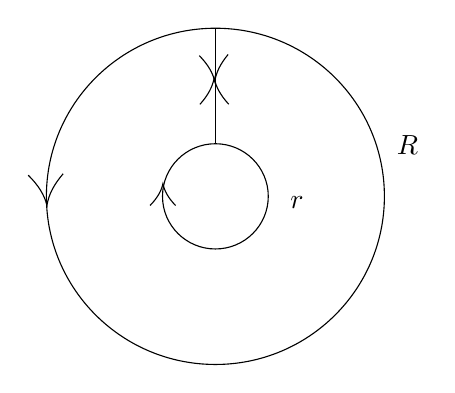
\begin{tikzpicture}[x=0.75pt,y=0.75pt,yscale=-1,xscale=1]
%uncomment if require: \path (0,467); %set diagram left start at 0, and has height of 467

%Shape: Ellipse [id:dp7827454042701263] 
\draw   (264.25,103) .. controls (264.25,58.26) and (300.7,22) .. (345.67,22) .. controls (390.64,22) and (427.1,58.26) .. (427.1,103) .. controls (427.1,147.74) and (390.64,184) .. (345.67,184) .. controls (300.7,184) and (264.25,147.74) .. (264.25,103) -- cycle ;
%Shape: Ellipse [id:dp2591539768992508] 
\draw   (320.19,103) .. controls (320.19,89) and (331.6,77.65) .. (345.67,77.65) .. controls (359.74,77.65) and (371.15,89) .. (371.15,103) .. controls (371.15,117) and (359.74,128.35) .. (345.67,128.35) .. controls (331.6,128.35) and (320.19,117) .. (320.19,103) -- cycle ;
%Straight Lines [id:da5441556171769937] 
\draw    (345.67,22) -- (345.67,77.65) ;


\draw   (272.31,92.13) .. controls (267.84,97.29) and (265.25,102.37) .. (264.52,107.38) .. controls (263.38,102.45) and (260.37,97.6) .. (255.5,92.81) ;
\draw   (314.22,107.37) .. controls (317.64,103.87) and (319.69,100.38) .. (320.39,96.88) .. controls (321.05,100.38) and (323.09,103.89) .. (326.48,107.41) ;
\draw   (351.8,34.66) .. controls (348.11,39.04) and (345.98,43.37) .. (345.38,47.63) .. controls (344.43,43.44) and (341.95,39.29) .. (337.92,35.22) ;
\draw   (338.21,58.69) .. controls (342.04,54.44) and (344.33,50.19) .. (345.08,45.96) .. controls (345.88,50.18) and (348.21,54.41) .. (352.1,58.62) ;

% Text Node
\draw (385,105.76) node  [align=left] {$\displaystyle r$};
% Text Node
\draw (438.17,78.2) node  [align=left] {$\displaystyle R$};


\end{tikzpicture}

\end{center}

b) Define the following functions:
\[
  g(z) = - \frac{1}{2\pi i}\int\limits_{C_{r}}\frac{f(\xi)}{\xi -z} \ d\xi, \ h(z) = \frac{1}{2\pi i}\int\limits_{C_{R}}\frac{f(\xi)}{\xi -z} \ d\xi
\]
 Consider first the case of the function $h$. We have that it is well defined at every point $v \notin C_{r}$. Let $|w| < R$ arbitrary. Fix an $\epsilon> 0$. For  $0 < \delta < \epsilon\left|\frac{\min_{C_{R}}|z-w|^{2}}{\max_{C_{R}}|f(z)|}\cdot\frac{1}{R}\right| $, we have for $k \in \bb{C}$ with $|k| < \delta$, the following string of manipulations:
  \begin{align*}
    & \frac{1}{2 \pi}\left| \ \int\limits_{\gamma} \frac{f(z)}{z-w}dz - \int\limits_{\gamma} \frac{f(z)}{z-w + k}dz \ \right| \leq \ \frac{1}{2\pi} \ \int\limits_{0}^{1} \frac{|kf(\gamma(t))|}{|(\gamma(t)-w)^{2} + (\gamma(t)-w)k|}\cdot |\gamma'(t)| dt \\
    \leq \ & \frac{1}{2 \pi}\int\limits_{0}^{1} \frac{\delta |f(\gamma(t))|}{|(\gamma(t)-w)^{2}|} \cdot |\gamma'(t)|dt \leq \delta \left|\frac{\max_{C_{R}} |f(z)|}{\min_{C_{R}}|z-w|^{2}}\right|\frac{1}{2\pi} \cdot 2 \pi r \leq \epsilon
  \end{align*}
  And so $h$ is continuous at every point in . Similar logic holds in showing $g$ is continuous as well. We now turn to showing that $h$ is holomorphic in the disk of radius less than $|R|$. Consider the following string of manipulations for $\epsilon \to 0$ in $\bb{C}$:
  \begin{align*}
    \lim_{\epsilon \to 0}\frac{1}{2\pi i}\frac{h(z+\epsilon)}{\epsilon} = \lim_{\epsilon\to 0} \frac{1}{2\pi i}\frac{1}{\epsilon}\int\limits_{C_{R}}\frac{f(w)}{(w - z) - \epsilon} - \frac{f(w)}{w-z} \ dw \\
    = \frac{1}{2\pi i}\lim_{\epsilon\to 0}\int\limits_{C_{R}}\frac{f(w)}{\epsilon} \frac{\epsilon}{(w-z)^{2} - \epsilon(w-z)} dw = \frac{1}{2\pi i}\int\limits_{C_{R}}\frac{f(w)}{(w-z)^{2}} dw 
  \end{align*}
  Which is defined at every point $z \notin C_{R}$, and so the function $h$ is holomorphic. Similar logic holds for $g$. Thus, we have that $f = g + h$. \\

  c) We have that $g$ is holomorphic in $\{|z| > r \}$, and so $q(z) = g(\frac{1}{z})$ is holomorphic in the region $\{0<|z| < \frac{1}{r}\}$. We have that $g$ is bounded for $|z| >> r$ by below:
  \[
    |g(z)| \leq \int\limits_{C_{r}} \frac{1}{2\pi}\frac{|f(w)|}{|w| - |r|} \ d|w| \max_{\xi \in C_{r}}(|f(\xi)|)\frac{1}{|w| - |r|} r
  \]
  This implies $q$ is bounded for $|z| << \frac{1}{r}$, i.e that it has a removable singularity at $0$. Thus, $q$ has a power series expansion valid in the disk $\{|z| < \frac{1}{r}\}$ as the one around $0$ must converge in compact subsets of this disk for every value less than $\frac{1}{r}$. Thus, we have that $q(z) = \sum_{n=0}^{\infty}c_{n}z^{n}$. For $|z| > r$ we have that $q(\frac{1}{z}) = g(z) = \sum_{n=0}^{\infty}c_{n}z^{-n}$ and this converges in compact subsets of $\{|z| > r\}$. We also know that $h$ has a power series expansion (say with coefficients $a_{n}$) valid in the disk of radius $R$. Thus, $g+h = \sum_{n=0}^{\infty}c_{n}z^{-n} + \sum_{k=0}^{\infty}a_{n}z^{n}$, a series converging in compact subsets of the annulus given above. This yields the claim. 
\end{proof}

\begin{exercise}
  Let $E \subset [0,1] \subset \bb{R} \subset \bb{C}$ denote the usual Cantor set $B$ the open disk of radius 2, $f: B \setminus E \to \bb{C}$ bounded and holomorphic. Show that $f$ admits a holomorphic extension to all of $B$.
\end{exercise}
\begin{proof}
  Denote the bound of $f$ by $C$. Let $C_{r}$ be the circle of radius $1.5$, i.e. the boundary of a disk containing the Cantor set. As before, we denote the function $h$ by:
  \[
    h(z) = \frac{1}{2\pi i}\int\limits_{C_{2}} \frac{f(w)}{w - z} \ dw
  \]
  Which is continuous and holomorphic in the ball of radius $1.5$ using an argument exactly parallel to the argument used in 2 b) to show the $h$ there satisfied the same properties. It thus suffices to show that $h(z)$ agrees with $f$ in the ball containing the Cantor set, as then $h$ provides the required extension to the Cantor set. Fix $ \epsilon > 0$, let $0 < a < 1.5$ arbitrary. We have that we may cover the Cantor set by $2^{N}$ nonintersecting balls of radius $\frac{1}{2\cdot 3^{N}}$, just by looking at ways to cover it using intervals in the real line. We select $N$ large such that $(2/3)^{N}\pi < \frac{a \epsilon}{2C}$ and such that $\frac{1}{2\cdot3^{N}} < \frac{a}{2}$, which we may do as $\frac{2^{N}}{3^{N}} \to 0$ as $N \to \infty$. Thus, we have $2^{N}$ nonintersecting balls $\{D_{i}\}_{i= 1,...,2^{N}}$ such that:
  \[
    f(z) = \frac{1}{2\pi i}\int\limits_{C_{r} - \sum D_{i}} \frac{f(w)}{w-z} dw
  \]
  Where the above Cauchy Integral Formula may be observed by iterating the decomposition process constructed in 1 a) for finitely many enclosed contours. Thus, we have that for any $z$ such that the distance between $z$ and the Cantor set is at least $a$:
  \[
    |f(z) - h(z)| \leq -\frac{1}{2\pi i} \int\limits_{\sum D_{i}}\frac{C}{|w - z|} dw \leq \int\limits_{\sum D_{i}}\frac{2C}{a} dw \leq (2/3)^{N}\pi \cdot \frac{2C}{a} \leq \epsilon
  \]
  In particular, as $\epsilon$ was arbitrary, $f$ and $h$ must agree on any point at a positive distance from the Cantor set. However, as the Cantor set is compact, this includes all of $B \setminus E$ and so $f$ and $h$ agree where $f$ is defined: this yields the claim. 
\end{proof}
\begin{exercise}
  a) Evaluate $\int\limits_{0}^{\infty}\frac{\sqrt{x}}{x^{2}+1} \ dx$. \\
  b) Evaluate $\int\limits_{0}^{2\pi}[\sin\theta]^{2k}d\theta$ for all integers $k\geq 1$
\end{exercise}
\begin{proof}
  a) Let $x \in \bb{R}^{+}$, and Log denote the logarithm along the principal branch cut in $\bb{C}$. Consider the following sequence of derivations:
  \[
    \lim_{\epsilon \to 0}\text{exp\{Log}(-x + i\epsilon)\frac{1}{2}\} - \text{exp\{Log}(- x - i\epsilon)\frac{1}{2}\} = e^{(log(x) + i\pi)/2} - e^{(log(x) - i\pi)/2} = \sqrt{x}(2i\sin\left(\frac{\pi}{2}\right)) = 2i \sqrt{x}
  \]
  Noting the above fact, we have that the integral above is equivalent to the integral:
  \begin{align*}
    2i\int\limits_{0}^{\infty}\frac{\sqrt{x}}{x^{2}+1} \ dx = \lim_{\epsilon \to 0}\int\limits_{0}^{\infty}\text{exp\{Log}(-z + i\epsilon)\frac{1}{2}\}\frac{1}{z^{2}+1+i\epsilon} - \text{exp\{Log}(- z - i\epsilon)\frac{1}{2}\}\frac{1}{z^{2}-i\epsilon + 1} \\
    = \lim_{\epsilon \to 0}\int\limits_{L_{1,\epsilon}}^{}\text{exp\{Log}(-z)\frac{1}{2}\}\frac{1}{z^{2}+1}dz + \int\limits_{L_{2,\epsilon}}^{}\text{exp\{Log}(-z)\frac{1}{2}\}\frac{1}{z^{2}+1} + \int\limits_{h_{\epsilon}}^{}\text{exp\{Log}(-z)\frac{1}{2}\frac{1}{z^{2}+1} 
  \end{align*}
  Where $L_{1, \epsilon}$ is the line $z = i\epsilon, \  Re(z) > -\frac{1}{2}$; $L_{2,\epsilon}$ is the line $z= - i\epsilon, \ Re(z) > -\frac{1}{2}$; and $h_{\epsilon}$ is the line from $-\frac{1}{2} - i\epsilon$ to $\frac{1}{2} + i\epsilon$, oriented as below:
  \begin{center}
    \tikzset{every picture/.style={line width=0.75pt}} %set default line width to 0.75pt        

\begin{tikzpicture}[x=0.75pt,y=0.75pt,yscale=-0.7,xscale=0.7]
%uncomment if require: \path (0,467); %set diagram left start at 0, and has height of 467

%Shape: Axis 2D [id:dp3276671432024534] 
\draw  (140.5,214.39) -- (499.5,214.39)(318.73,57) -- (318.73,370) (492.5,209.39) -- (499.5,214.39) -- (492.5,219.39) (313.73,64) -- (318.73,57) -- (323.73,64)  ;
%Straight Lines [id:da25973421256512275] 
\draw    (496.77,170.52) -- (295.1,170.31) ;


%Straight Lines [id:da2595336765420049] 
\draw    (496.77,259.79) -- (295.1,259.58) ;


%Straight Lines [id:da7577891192245878] 
\draw    (295.1,259.58) -- (295.1,170.31) ;


\draw   (392.25,161.68) -- (400.89,170.5) -- (392.25,179.32) ;
\draw   (395.57,268.14) -- (386.7,259.6) -- (395.09,250.51) ;
\draw   (286.99,222.01) -- (294.97,212.52) -- (303.4,221.56) ;
%Straight Lines [id:da5146530603443025] 
\draw    (368.5,247) -- (369.08,182.31) ;
\draw [shift={(369.1,180.31)}, rotate = 450.51] [color={rgb, 255:red, 0; green, 0; blue, 0 }  ][line width=0.75]    (10.93,-3.29) .. controls (6.95,-1.4) and (3.31,-0.3) .. (0,0) .. controls (3.31,0.3) and (6.95,1.4) .. (10.93,3.29)   ;

%Straight Lines [id:da7549206742958066] 
\draw    (369.1,180.31) -- (368.52,245) ;
\draw [shift={(368.5,247)}, rotate = 270.51] [color={rgb, 255:red, 0; green, 0; blue, 0 }  ][line width=0.75]    (10.93,-3.29) .. controls (6.95,-1.4) and (3.31,-0.3) .. (0,0) .. controls (3.31,0.3) and (6.95,1.4) .. (10.93,3.29)   ;

%Curve Lines [id:da11328702918370803] 
\draw    (318.73,214.39) .. controls (348.5,196) and (311.5,231) .. (341.5,216) ;


%Curve Lines [id:da5342085594115376] 
\draw    (341.5,216) .. controls (371.27,197.61) and (341.5,227) .. (364.27,217.61) ;


%Curve Lines [id:da8402426569180517] 
\draw    (364.27,217.61) .. controls (396.5,196) and (363.5,229) .. (391.5,216) ;


%Curve Lines [id:da1418013010733279] 
\draw    (391.5,216) .. controls (421.27,197.61) and (388.73,229.39) .. (418.73,214.39) ;


%Curve Lines [id:da5521259064148651] 
\draw    (418.73,214.39) .. controls (448.5,196) and (415.5,230) .. (445.5,215) ;


%Curve Lines [id:da44119921523478967] 
\draw    (445.5,215) .. controls (475.27,196.61) and (442.27,230.61) .. (472.27,215.61) ;


%Curve Lines [id:da8240292487439884] 
\draw    (472.27,215.61) .. controls (502.04,197.21) and (464.5,231) .. (494.5,216) ;



% Text Node
\draw (362.92,277.78) node  [align=left] {$\displaystyle L_{2,\epsilon }$};
% Text Node
\draw (365.95,154.64) node  [align=left] {$\displaystyle L_{1,\epsilon }$};
% Text Node
\draw (283.65,194.79) node  [align=left] {$\displaystyle h_{\epsilon }$};
% Text Node
\draw (389,198) node  [align=left] {$\displaystyle 2\epsilon $};


\end{tikzpicture}
\end{center}
With the preimage of the branch cut along the negative real axis taken to a branch cut along the positive real axis. Thus, it suffices to compute the limit of integrals along the following paths:
\begin{center}
  \tikzset{every picture/.style={line width=0.75pt}} %set default line width to 0.75pt        

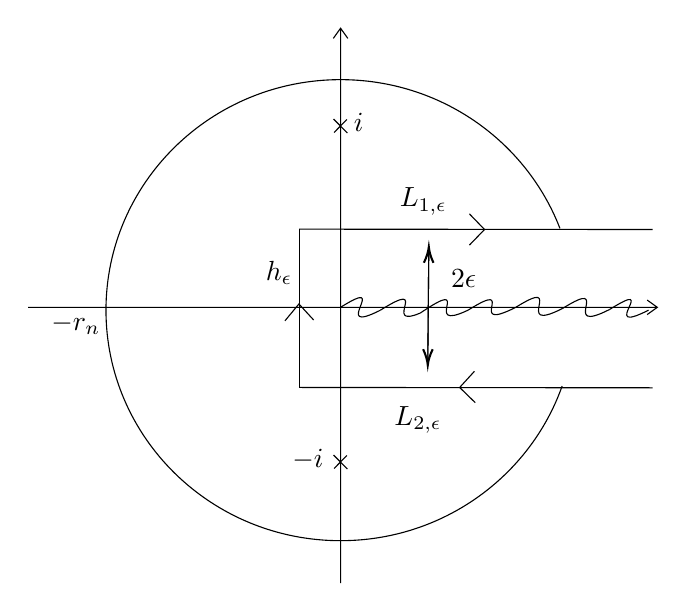
\begin{tikzpicture}[x=0.75pt,y=0.75pt,yscale=-0.7,xscale=0.7]
%uncomment if require: \path (0,467); %set diagram left start at 0, and has height of 467

%Shape: Axis 2D [id:dp3276671432024534] 
\draw  (122.5,227.09) -- (555.5,227.09)(337.47,35) -- (337.47,417) (548.5,222.09) -- (555.5,227.09) -- (548.5,232.09) (332.47,42) -- (337.47,35) -- (342.47,42)  ;
%Straight Lines [id:da25973421256512275] 
\draw    (552.21,173.54) -- (308.97,173.29) ;


%Straight Lines [id:da2595336765420049] 
\draw    (552.21,282.49) -- (308.97,282.24) ;


%Straight Lines [id:da7577891192245878] 
\draw    (308.97,282.24) -- (308.97,173.29) ;


\draw   (426.15,162.76) -- (436.56,173.52) -- (426.15,184.28) ;
\draw   (430.15,292.69) -- (419.45,282.26) -- (429.57,271.17) ;
\draw   (299.18,236.39) -- (308.81,224.8) -- (318.97,235.84) ;
%Straight Lines [id:da5146530603443025] 
\draw    (397.5,266.88) -- (398.2,187.49) ;
\draw [shift={(398.22,185.49)}, rotate = 450.51] [color={rgb, 255:red, 0; green, 0; blue, 0 }  ][line width=0.75]    (10.93,-3.29) .. controls (6.95,-1.4) and (3.31,-0.3) .. (0,0) .. controls (3.31,0.3) and (6.95,1.4) .. (10.93,3.29)   ;

%Straight Lines [id:da7549206742958066] 
\draw    (398.22,185.49) -- (397.51,264.89) ;
\draw [shift={(397.5,266.88)}, rotate = 270.51] [color={rgb, 255:red, 0; green, 0; blue, 0 }  ][line width=0.75]    (10.93,-3.29) .. controls (6.95,-1.4) and (3.31,-0.3) .. (0,0) .. controls (3.31,0.3) and (6.95,1.4) .. (10.93,3.29)   ;

%Curve Lines [id:da11328702918370803] 
\draw    (337.47,227.09) .. controls (373.37,204.64) and (328.75,247.36) .. (364.93,229.05) ;


%Curve Lines [id:da5342085594115376] 
\draw    (364.93,229.05) .. controls (400.84,206.6) and (364.93,242.48) .. (392.4,231.01) ;


%Curve Lines [id:da8402426569180517] 
\draw    (392.4,231.01) .. controls (431.27,204.64) and (391.47,244.92) .. (425.24,229.05) ;


%Curve Lines [id:da1418013010733279] 
\draw    (425.24,229.05) .. controls (461.15,206.6) and (421.9,245.4) .. (458.08,227.09) ;


%Curve Lines [id:da5521259064148651] 
\draw    (458.08,227.09) .. controls (493.99,204.64) and (454.19,246.14) .. (490.37,227.83) ;


%Curve Lines [id:da44119921523478967] 
\draw    (490.37,227.83) .. controls (526.28,205.38) and (486.47,246.88) .. (522.66,228.57) ;


%Curve Lines [id:da8240292487439884] 
\draw    (522.66,228.57) .. controls (558.56,206.12) and (513.29,247.36) .. (549.47,229.05) ;


%Shape: Arc [id:dp9395126304282921] 
\draw  [draw opacity=0] (489.98,281.27) .. controls (468.01,343.24) and (408.02,387.71) .. (337.47,387.71) .. controls (248.3,387.71) and (176.01,316.68) .. (176.01,229.05) .. controls (176.01,141.43) and (248.3,70.39) .. (337.47,70.39) .. controls (406.47,70.39) and (465.36,112.93) .. (488.47,172.77) -- (337.47,229.05) -- cycle ; \draw   (489.98,281.27) .. controls (468.01,343.24) and (408.02,387.71) .. (337.47,387.71) .. controls (248.3,387.71) and (176.01,316.68) .. (176.01,229.05) .. controls (176.01,141.43) and (248.3,70.39) .. (337.47,70.39) .. controls (406.47,70.39) and (465.36,112.93) .. (488.47,172.77) ;
\draw   (332.64,97.51) -- (342.17,107.08)(341.82,97.79) -- (332.99,106.79) ;
\draw   (332.64,328.77) -- (342.17,338.34)(341.82,329.06) -- (332.99,338.06) ;

% Text Node
\draw (390.77,304.45) node  [align=left] {$\displaystyle L_{2,\epsilon }$};
% Text Node
\draw (394.42,154.17) node  [align=left] {$\displaystyle L_{1,\epsilon }$};
% Text Node
\draw (295.15,203.16) node  [align=left] {$\displaystyle h_{\epsilon }$};
% Text Node
\draw (422.22,207.08) node  [align=left] {$\displaystyle 2\epsilon $};
% Text Node
\draw (155.29,238.81) node  [align=left] {$\displaystyle -r_{n}$};
% Text Node
\draw (349.99,99.88) node  [align=left] {$\displaystyle i$};
% Text Node
\draw (315,331.94) node  [align=left] {$\displaystyle -i$};

\end{tikzpicture}
\end{center}
Where $r_{n}$ can be taken to be arbitrarily large: as the length of the arc above grows linearly with respect to $r$, and the function decays at an exponential rate greater than $1$ as distance from the origin increases, we have that the limit of the integrals over these arcs must converge to $0$, implying that the limit of the sequence of integrals above for some $r_{n} \to \infty$ must converge to the integral over $L_{2,\epsilon} + h_{\epsilon} + L_{1,\epsilon}$. Thus, it suffices to check the values of these integrals. The function $\text{exp\{Log}(-z)\frac{1}{2}\}\frac{1}{z^{2}+1}$ has two simple poles at $i$ and $-i$. The value of any such integral, then, is the sum of the residues at these poles multiplied by $2\pi i$. Checking at $i$, we have:
\[
  \lim_{z \to i} \ (z-i) \cdot \text{exp\{Log}(-z)\frac{1}{2}\}\frac{1}{z^{2}+1} = \text{exp\{Log}(-i)\frac{1}{2}\}\frac{1}{2i} = \frac{1}{2i}e^{-i\pi/4}
\]
Similarly checking at $-i$, we have:
\[
  \lim_{z \to i} \ (z+i) \cdot \text{exp\{Log}(-z)\frac{1}{2}\}\frac{1}{z^{2}+1} = \text{exp\{Log}(i)\frac{1}{2}\}\frac{1}{2i} = \frac{1}{-2i}e^{i\pi/4}
\]
The value of any given integral then, is:
\[
  \pi \cdot (e^{-i\pi/4}- e^{i\pi/4}) = \frac{2i}{\sqrt{2}} \pi
\]
Thus, the value of the integral
\[
  \int\limits_{L_{1,\epsilon}}^{}\text{exp\{Log}(-z)\frac{1}{2}\}\frac{1}{z^{2}+1}dz + \int\limits_{L_{2,\epsilon}}^{}\text{exp\{Log}(-z)\frac{1}{2}\}\frac{1}{z^{2}+1} + \int\limits_{h_{\epsilon}}^{}\text{exp\{Log}(-z)\frac{1}{2}\frac{1}{z^{2}+1} 
\]
Is given by $\frac{2i}{\sqrt{2}} \pi$ for all $\epsilon$, and thus in the limit we get that the desired integral has the value below:
\[
  2i \int\limits_{0}^{\infty}\frac{\sqrt{x}}{x^{2}+1} dx = \frac{2i}{\sqrt{2}}\pi \implies \int\limits_{0}^{\infty}\frac{\sqrt{x}}{x^{2}+1} dx = \frac{\pi}{\sqrt{2}}
\]

b) Using the identity $2 i \sin \theta =  e^{i\theta} - e^{-i\theta}$ we have that the integral above is:
\begin{align*}
 & 2^{-2k}(-1)^{k}\int\limits_{0}^{2\pi}[e^{i\theta} - e^{-i\theta}]^{2k} d\theta = 2^{-2k}(-1)^{k} \int\limits_{0}^{2\pi}\left(\sum_{j=0}^{-2k}\frac{2k!}{j! (2k-j)!}e^{2i(j-k)\theta}\right) d\theta \\
= \ & 2^{-2k}(-1)^{k} \sum_{j=0}^{2k}\left(\frac{2k!}{j! (2k-j)!} \int\limits_{0}^{2\pi}e^{2i(j-k)\theta}d\theta\right) = 2^{1-2k}(-1)^{k}\pi \frac{2k!}{k! \cdot k!}
  \end{align*}
\end{proof}

\begin{exercise}
  a) Evaluate \[ \int\limits_{\gamma}e^{2\pi n z}z^{-s}dz\] for each integer $n\geq 1$. \\
  b) Show that
  \[
    \int\limits_{\gamma}\frac{e^{2 \pi N z}}{e^{-2\pi z} - 1} z^{-s}dz 
  \]
  converges to zero as $N \to \infty$. \\
  c) Deduce the functional equation for $\zeta$. 
\end{exercise}
\begin{proof}
  Consider the following diagram:
  \begin{center}
    \begin{tikzpicture}[x=0.75pt,y=0.75pt,yscale=-0.7,xscale=0.7]
%uncomment if require: \path (0,467); %set diagram left start at 0, and has height of 467

%Shape: Axis 2D [id:dp3276671432024534] 
\draw  (89.03,227.5) -- (522.03,227.5)(304,35.41) -- (304,417.41) (515.03,222.5) -- (522.03,227.5) -- (515.03,232.5) (299,42.41) -- (304,35.41) -- (309,42.41)  ;
%Straight Lines [id:da5146530603443025] 
\draw    (143.5,268.88) -- (143.5,248) ;
\draw [shift={(143.5,246)}, rotate = 450.01] [color={rgb, 255:red, 0; green, 0; blue, 0 }  ][line width=0.75]    (10.93,-3.29) .. controls (6.95,-1.4) and (3.31,-0.3) .. (0,0) .. controls (3.31,0.3) and (6.95,1.4) .. (10.93,3.29)   ;

%Straight Lines [id:da7549206742958066] 
\draw    (145.22,179.49) -- (145.48,208) ;
\draw [shift={(145.5,210)}, rotate = 269.47] [color={rgb, 255:red, 0; green, 0; blue, 0 }  ][line width=0.75]    (10.93,-3.29) .. controls (6.95,-1.4) and (3.31,-0.3) .. (0,0) .. controls (3.31,0.3) and (6.95,1.4) .. (10.93,3.29)   ;

%Curve Lines [id:da11328702918370803] 
\draw    (127.47,227.09) .. controls (163.37,204.64) and (118.75,247.36) .. (154.93,229.05) ;


%Curve Lines [id:da5342085594115376] 
\draw    (154.93,229.05) .. controls (190.84,206.6) and (154.93,242.48) .. (182.4,231.01) ;


%Curve Lines [id:da8402426569180517] 
\draw    (182.4,231.01) .. controls (221.27,204.64) and (181.47,244.92) .. (215.24,229.05) ;


%Curve Lines [id:da1418013010733279] 
\draw    (215.24,229.05) .. controls (251.15,206.6) and (211.9,245.4) .. (248.08,227.09) ;


%Curve Lines [id:da5521259064148651] 
\draw    (248.08,227.09) .. controls (283.99,204.64) and (244.19,246.14) .. (280.37,227.83) ;


%Curve Lines [id:da44119921523478967] 
\draw    (280.37,227.83) .. controls (316.28,205.38) and (268.47,245.88) .. (304.66,227.57) ;


%Straight Lines [id:da5904464354263184] 
\draw    (151.5,127) -- (409.47,227.09) ;


%Straight Lines [id:da9474289874184498] 
\draw    (155.5,332) -- (409.47,227.09) ;


%Curve Lines [id:da4239569335310114] 
\draw    (99.5,228) .. controls (135.41,205.55) and (91.28,245.4) .. (127.47,227.09) ;


%Straight Lines [id:da6114300328295577] 
\draw    (153.5,176) -- (409.47,227.09) ;


%Straight Lines [id:da17255105006786375] 
\draw    (157.5,268) -- (409.47,227.09) ;



% Text Node
\draw (417,206) node  [align=left] {$\displaystyle \epsilon $};
% Text Node
\draw (231,128) node  [align=left] {$\displaystyle L_{1}$};
% Text Node
\draw (179,194) node  [align=left] {$\displaystyle L_{1} '$};
% Text Node
\draw (177,276) node  [align=left] {$\displaystyle L_{2} '$};
% Text Node
\draw (189,339) node  [align=left] {$\displaystyle L_{2}$};


\end{tikzpicture}
  \end{center}
  By an argument involving showing that the regions bounded by $L_{1}, L_{1}'$ are regions over which the function in consideration is holomorphic and taking the limit of triangles along $L_{1}, L_{1}'$ and seeing that the integral over the base decays as it goes to infinity, we see that the integral over $L_{1}$ must be the same as $L_{1}'$ and likewise for $L_{2}$. Using this rationale, we may ``collapse'' the contour $\gamma$ onto the negative real axis by taking the limit of integrals along straight paths converging to the negative real axis along the upper and lower half planes: we see that these integrals have continuously defined limits along different branch cuts of the logarithm, and so we may evaluate this contour collapsed onto the real axis as:
  \begin{align*}
    & \int\limits_{\gamma}^{}e^{2\pi n z}z^{-s}dz = \int\limits_{0}^{\infty}e^{-2 \pi n t - i\pi s}t^{-s} dt - \int\limits_{0}^{\infty}t^{-s}e^{-2\pi n t + i \pi s} dt \\
    = \ &  \frac{e^{-i \pi s}}{(2\pi n)^{1-s}} \Gamma(1-s) - \frac{e^{i \pi s}}{(2\pi n)^{1-s}} \Gamma(1-s) = \Gamma(1-s)(2\pi n)^{1-s}(e^{-i\pi s} - e^{-i \pi s}) \\
        = \ & \Gamma(1-s)(2\pi n)^{1-s} \cdot 2 i \sin(\pi s)
  \end{align*}
  b) Using the same argument as earlier, we may rewrite this integral as the following:
  \[
    \int\limits_{0}^{\infty}\frac{e^{-2\pi N t}}{e^{2\pi t} - 1} t^{-s}( e^{-i\pi s}  - e^{i \pi s}) dt = (2 \pi)^{s-1} \int\limits_{0}^{\infty}\frac{e^{-Nu}}{e^{u} - 1} u^{-s} du    
    \]
    Fix $\epsilon> 0$. We have that:
    \[
      |(2\pi)^{Re(s) - 1}|\int\limits_{0}^{\infty}\left|\frac{e^{-Nu}}{e^{u}-1} u^{-s}\right| \ d|u| \leq \int\limits_{0}^{\infty}\left|\frac{u^{-s}}{e^{u}-1}\right| \ d|u| \leq \int\limits_{0}^{\infty}\frac{u^{ - Re(s)}}{e^{u}-1 } du   
      \]
      And as the term on the left is a convergent integral for $Re(s) < 0$ which is our condition, we have that we may select $x_{0}$ small such that
      \[
        \int\limits_{0}^{x_{0}}\frac{u^{-Re(s)}}{e^{u}-1} du \leq \frac{\epsilon(2\pi)^{1-Re(s)}}{3}
      \]
      And $M$ large such that
      \[
        \int\limits_{M}^{\infty}\frac{u^{-Re(s)}}{e^{u}-1} du \leq \frac{\epsilon(2\pi)^{1-Re(s)}}{3}
      \]
      In the region $[x_{0}, M]$, which is compact, we have that $\frac{e^{-Nu}}{e^{u}-1}$ converges uniformly to $0$ as $N \to \infty$, and thus we may select $N$ large such that
      \[
        \int\limits_{x_{0}}^{M}\frac{|e^{-Nu}u^{-Re(s)}|}{|e^{u}-1|} du \leq \frac{\epsilon(2\pi)^{1-Re(s)}}{3}
      \]

      Adding the above integrals together, we have that:
      \[
        \int\limits_{0}^{\infty}\left|\frac{e^{-Nu}}{e^{u}-1} u^{-s}\right| \ d|u| < \epsilon
      \]
      As $N \to \infty$, and as $\epsilon$ was arbitrary we have that the integral above converges to zero as $N \to \infty$, yielding the claim. 
    c) We may write $\frac{1}{e^{-2\pi z} - 1} = \frac{e^{2 \pi N z}}{e^{- 2 \pi z } - 1} + \sum_{n=1}^{N} e^{2 \pi n z}$ for large $N$. Making this substitution in our expression for $\zeta(s)$, we have:
    \begin{align*}
      & \zeta(s) = \frac{1}{2i \cos(\pi s / 2)} \int\limits_{\gamma} \frac{z^{-s}dz}{e^{-2\pi z } - 1} = \frac{1}{2i \cos(\pi s / 2)} \left( \sum_{n=0}^{N} \int\limits_{\gamma} e^{2\pi n z}z^{-s}dz \right) + E(N) \\
      = \ & \frac{1}{2i \cos(\pi s /2)} \sum_{n=0}^{N}\Gamma(1-s)(2\pi n)^{1-s}2i \sin(\pi s) + E(N) = \sum_{n=0}^{N}\Gamma(1-s)(2\pi n)^{1-s} \cdot 2 \sin(\pi s/2) + E(N)
    \end{align*}
    As $N$ goes to infinity the error term $E(N)$ goes to zero and the sum on the right converges to the sum below:
    \[
      \zeta(s) = \Gamma(1-s) 2^{-s}\pi^{1-s} \sin(\pi s /2) \sum_{n=0}^{\infty}n^{1-s} = 2^{-s} \pi^{1-s}\sin(\pi s/2) \Gamma(1-s) \zeta(1-s) 
      \]
\end{proof}
\end{document}

